\documentclass[a4paper,12pt]{article}
\usepackage{amsmath,amssymb,amsfonts,amsthm}
\usepackage{tikz}
\usepackage [utf8x] {inputenc}
\usepackage [T2A] {fontenc} 
\usepackage[russian]{babel}
\usepackage{cmap} 
\usepackage{ gensymb }
% Так ссылки в PDF будут активны
\usepackage[unicode]{hyperref}
\usepackage{ textcomp }
\usepackage{indentfirst}
\usepackage[version=3]{mhchem}

% вы сможете вставлять картинки командой \includegraphics[width=0.7\textwidth]{ИМЯ ФАЙЛА}
% получается подключать, как минимум, файлы .pdf, .jpg, .png.
\usepackage{graphicx}
% Если вы хотите явно указать поля:
\usepackage[margin=1in]{geometry}
% Или если вы хотите задать поля менее явно (чем больше DIV, тем больше места под текст):
% \usepackage[DIV=10]{typearea}

\usepackage{fancyhdr}

\newcommand{\bbR}{\mathbb R}%теперь вместо длинной команды \mathbb R (множество вещественных чисел) можно писать короткую запись \bbR. Вместо \bbR вы можете вписать любую строчку букв, которая начинается с '\'.
\newcommand{\eps}{\varepsilon}
\newcommand{\bbN}{\mathbb N}
\newcommand{\dif}{\mathrm{d}}

\newtheorem{Def}{Определение}


\pagestyle{fancy}
\makeatletter % сделать "@" "буквой", а не "спецсимволом" - можно использовать "служебные" команды, содержащие @ в названии
\fancyhead[L]{\footnotesize Лабораторные работы по общей физике}%Это будет написано вверху страницы слева
\fancyhead[R]{\footnotesize ФУПМ МФТИ}
%\fancyfoot[L]{\footnotesize \@author}%имя автора будет написано внизу страницы слева
\fancyfoot[R]{\thepage}%номер страницы —- внизу справа
\fancyfoot[C]{}%по центру внизу страницы пусто

\renewcommand{\maketitle}{%
	\noindent{\bfseries\scshape\large\@title\ \mdseries\upshape}\par
	\noindent {\large\itshape\@author}
	\vskip 2ex}
\makeatother
\def\dd#1#2{\frac{\partial#1}{\partial#2}}


\title{1.3. Изучение рассеяния медленных электронов на атомах (эффект Рамзауэра)}
\author{Хурсик Екатерина} 

\begin{document}	
\maketitle


\section{Цель работы}
    Исследовать энергетическую зависимость вероятности рассеяния электронов
    атомами ксенона, определить энергии электронов, при которых наблюдается 
    "просветление" ксенона, и оценить размер его внешней электронной оболочки.
\section{Метод}

    Эффект Рамзауэра нельзя объяснить с позиций классической теории. С квантовой же точки зрения картина рассеяния выглядит следующим образом. Внутри атома потенциальная энергия налетающего электрона отлична от нуля, скорость электрона меняется, становясь равной $v'$ в соответсвии с законом сохранения энергии:
    \begin{equation}
    E = \frac{mv^2}{2} = \frac{mv'^2}{2} + U
    \end{equation}

    а значит, изменяется и длина его волны де Бройля. Таким образом, по отношению к электронной волне атом ведет себя как преломляющая среда с относительным показателем преломления:

    \begin{equation}
    n = \frac{\lambda}{\lambda'} = \sqrt{1 - \frac{U}{E}}
    \end{equation}

    Решение задачи о рассеянии электрона на сферическом потенциале достаточно громоздко. Поэтому рассмотрим более простое одномерное приближение: электрон рассеивается на потенциальной яме конечной глубины. Уравнение Шрёдингера в этом случае имеет вид:
    \begin{equation}
    \psi'' + k^2\psi = 0 \qquad k^2 = \begin{cases}
    k_1^2  = \frac{2mE}{\hbar^2} \\
    k_2 = \frac{2m(E+U_0)}{\hbar^2}
    \end{cases}
    \end{equation}

    Коэффициент прохождения равен отношению квадратов амплитуд прошедшей и падающей волн и определяется выражением:
    \begin{equation}
    D = \frac{16k_1^2k_2^2}{16k_1^2k_2^2 + 4(k_1^2-k_2^2)^2\sin^2(k_2l)}
    \end{equation}

    Видно, что коэффициент прохождения частицы над ямой, в зависимости от её энергии, имеет вид чередующихся максимумов и минимумов. В частности, если $k_2l = \pi$, то коэффициент прохождения равен 1, т.е. отраженная волна отсутствует, и электрон беспрепятственно проходит через атом. Этот эффект является квантовым аналогом просветления оптики. Таким образом, коэффициент прохождения электронов максимален при условии:
    \begin{equation}
    k_2l = \sqrt{\frac{2m(E+U_0)}{\hbar^2}}l = \pi n
    \end{equation}
    Прошедшая волна 1 усилится волной 2, если геометрическая разность хода между ними $\Delta = 2l = \lambda'$, что соответствует условию первого интерференционного максимума, т.е.
    \begin{equation}
    2l = \frac{h}{\sqrt{2m(E_1 + U_0)}}
    \end{equation}
    C другой стороны, прошедшая волна ослабится, если $2l = \frac{3}{2}\lambda'$, т.е.
    \begin{equation}
    2l = \frac{3}{2}\frac{h}{\sqrt{2m(E_2+U_0)}}
    \end{equation}
    Решая эти уравнения совместно можно исключить $U_0$ и найти эффективный размер атома $l$:
    \begin{equation}
        l = \frac{h\sqrt{5}}{\sqrt{2m(E_2-E_1)}}
    \end{equation}
    Понятно, что энергии $E_1$, $E_2$ соответсвуют энергия электронов, прошедших разность потенциалов $V_1$ и $V_2$.
    Кроме того, можно оценить эффективную глубину потенциальной ямы атома:
    \begin{equation}
    U_0 =\frac{4}{5}E_2 - \frac{9}{5}E_1
    \end{equation}

    Теперь рассмотрим ВАХ тиратрона. Она имеет вид:
    $$
    I_a = I_0e^{-C\omega(V)}, C = Ln_a\Delta_a
    $$
    где $I_0 = eN_0$ --- ток катода, $I_a = eN_a$ --- анодный ток, $\Delta_a$ --- площадь поперечного сечения атома, $n_a$ --- концентрация атомов газа в лампе, $L$ --- расстояние от катода до анода, $\omega(V)$ --- вероятность рассеяния электрона на атоме как функция от ускоряющего напряжения. По измеренной ВАХ тиратрона можно определить зависимость вероятности рассеяния электрона от его энергии из соотношения:
    \begin{equation}
    \omega(V) = -\frac{1}{C}\ln\frac{I_a}{I_0}
    \end{equation}
    %********************************************************************
    В 1921г. Карл Рамзауэр исследовал зависимость поперечных сечений упругого
    рассеяния электронов на атомах аргона. В результате этих исследований было обнаружено
    явление, получившее название \textit{эффекта Рамзауэра}.

    Эффективное сечение реакции (поперечное сечение) -- это величина, характеризующая вероятность перехода
    системы двух сталкивающихся частиц в результате их рассеяния (упругого или
    неупругого) в определенное конечное состояние. Сечение $\sigma$ это отношение
    числа таких переходов $N$ в единицу времени к плотности потока $nv$ рассеиваемых
    частиц, падающих на мишень, т.е. к числу частиц, попадающих в единицу времени
    на единичную площадку, перпендикулярную к их скорости $\upsilon$

    \begin{equation}
    \sigma = \frac{N}{nv}
    \end{equation}


    Качественно результат экспериментов Рамзауэра при энергии электронов порядка десятков
    электрон-вольт на аргоне показан на рис.1. 

    \begin{figure}[h!]
        \begin{center}
            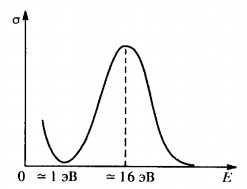
\includegraphics[width=0.5\linewidth]{2020-12-10-1.jpg}
            \caption{результаты измерения упругого рассеяния электронов в аргоне}
        \end{center}
    \end{figure}
    \pagebreak
    
    По мере уменьшения энергии электрона от нескольких
    десятков электрон-вольт поперечное сечение его упругого рассеяния растёт: чем меньше скорость
    электрона, тем медленнее он "проскакивает" мимо атома, тем больше вероятность этого
    взаимодействия, т.е. сечение реакции. Однако в эксперименте наблюдалось, что при
    энергиях меньше 16эВ сечение начинает уменьшаться, а при $E\approx 1$ эВ практически
    равно нулю, т.е. аргон становится прозрачным для электронов. При дальнейшем уменьшении
    энергии электронов сечение рассеяния опять начинает возрастать.

    \begin{figure}[h!]
        \begin{center}
            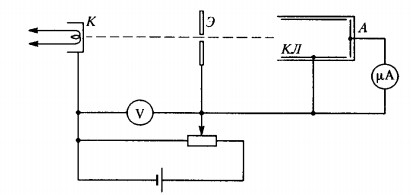
\includegraphics[width=0.5\linewidth]{2020-12-10-2.jpg}
            \caption{Схема эксперимента Рамзауэра}
        \end{center}
    \end{figure}
    \pagebreak

    
\end{document}

